\chapter{Web interface}
\label{chap:web-interface}

  In addition to the command-line programs, the project provides a web
  interface for prototyping queries, and quick data reporting.  With the
  web interface you can:
  \begin{itemize}
  \item Write and execute SPARQL queries;
  \item Combine multiple SPARQL endpoints;
  \item Configure ``projects'' to subset data.
  \end{itemize}

\section{Configuring the web interface}
\label{sec:configuring-sg-web}

  Before the web interface can be started, a few parameters have to be
  configured.  This is done through an XML file.  The following example
  displays all options, except for the authentication part, which is
  discussed separately in section \ref{sec:authentication}
  {\color{LinkGray}`\nameref{sec:authentication}'}.

\begin{siderules}
\begin{verbatim}
<?xml version="1.0" encoding="utf-8"?>
<web-interface>
  <fork>0</fork>
  <bind-address>127.0.0.1</bind-address>
  <port>8080</port>
  <authentication>
    <!-- Either LDAP settings, or single-user authentication -->
  </authentication>
</web-interface>
\end{verbatim}
\end{siderules}

\subsection{To fork or not to fork}

  The \texttt{fork} property can be either \texttt{0} to keep the
  \texttt{sg-web} process in the foreground of your shell, or
  \texttt{1} to run the \texttt{sg-web} process as a daemon.

\subsection{Bind address and port}

  Because web services are popular these days, \texttt{sg-web} can be configured
  to bind on an arbitrary address and an arbitrary port.

\subsection{Authentication}
\label{sec:authentication}

  There are two ways to configure authentication.  For single-user deployments
  or environments that lack an LDAP service, a preconfigured username and
  password can be set.  For a multi-user deployment, the web interface can be
  configured to use an LDAP server.

\subsubsection{Single-user configuration}

  The simplest form of authentication is the ``single-user configuration''.
  Make sure the configuration file is only readable by yourself, as the
  credentials are stored in plain text.  The following example shows how
  to configure ``single-user authentication'':

\begin{siderules}
\begin{verbatim}
<?xml version="1.0" encoding="utf-8"?>
<web-interface>
  ...
  <authentication>
    <single-user>
      <username>user</username>
      <password>test</password>
    </single-user>>
  </authentication>
</web-interface>
\end{verbatim}
\end{siderules}

\subsubsection{LDAP authentication example}

  To configure LDAP, three parameters must be specified: the URI to the LDAP
  service (1), the ``organizational unit'' (2), and the ``domain'' (3).  The
  username is used as the ``common name''.

  The following example shows how to configure LDAP authentication:

\begin{siderules}
\begin{verbatim}
<?xml version="1.0" encoding="utf-8"?>
<web-interface>
  ...
  <authentication>
    <ldap>
      <uri>ldap://example.local</uri>
      <organizational-unit>People</organizational-unit>
      <domain>department.organization.tld</domain>
    </ldap>
  </authentication>
</web-interface>
\end{verbatim}
\end{siderules}

\section{Running the web interface}

  The web interface can be started using the \texttt{sg-web} command:

\begin{siderules}
\begin{verbatim}
sg-web --configuration-file=file.xml
\end{verbatim}
\end{siderules}

  $\ldots{}$ where \texttt{file.xml} is a configuration file as
  discussed in section \ref{sec:configuring-sg-web}
  {\color{LinkGray}`\nameref{sec:configuring-sg-web}'}.

\section{Configuring connections}
\label{sec:configure-connections}

  The first useful step is to configure a connection to a SPARQL endpoint.

  \begin{figure}[h]
    \begin{center}
      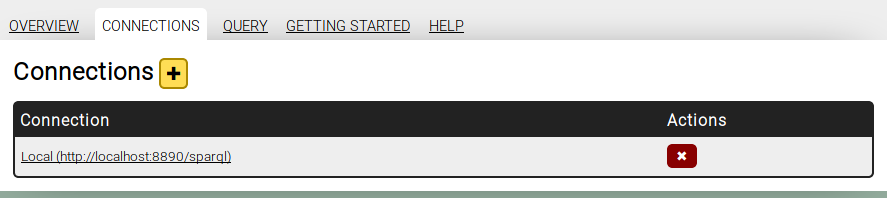
\includegraphics[width=1.0\textwidth]{figures/web-connections.png}
    \end{center}
    \caption{The \emph{connections} page enables users to configure accessible
      SPARQL endpoints.  Adding a connection here will provide an option to
      query it on the \emph{query} page.}
    \label{fig:web-connections}
  \end{figure}

  When providing a username and password for a connection, it will attempt
  to connect using \emph{digest authentication}.

\section{Managing projects}

  When interacting with large datasets, it may be useful to confine queries to
  a subset of the dataset.  On the \emph{projects} page, subsets can be made
  based on \emph{sample names}.  These sample names are automatically extracted
  from VCF files, and can also be extracted from tabular data.

  Marking a project as ``active'' indicates that queries executed using the web
  interface relate to that project.  See also section \ref{sec:query-history}
  {\color{LinkGray}`\nameref{sec:query-history}'}.

\section{Executing queries}

  After configuring at least one endpoint, it can be chosen on the \emph{query}
  page to execute a query against it.

  \begin{figure}[h]
    \begin{center}
      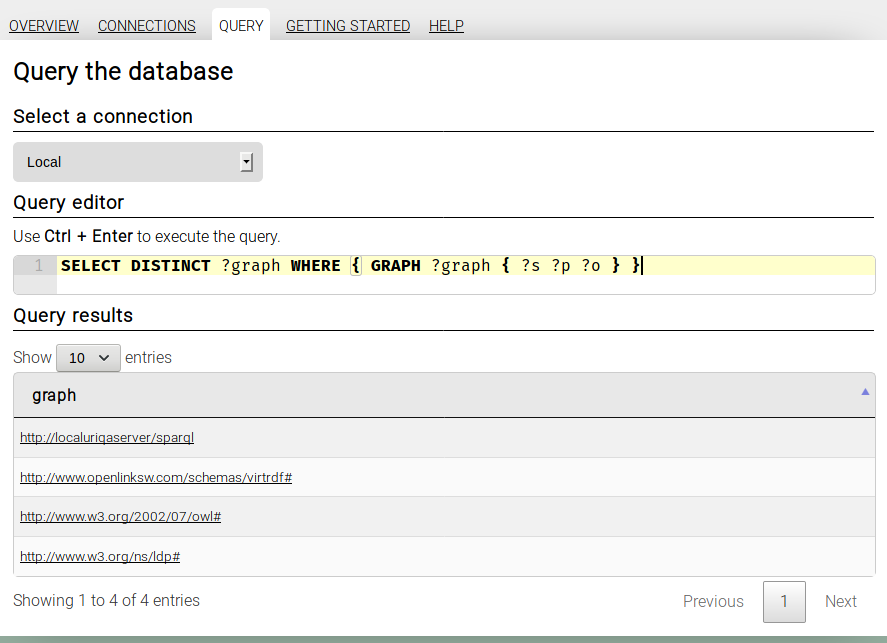
\includegraphics[width=1.0\textwidth]{figures/web-query.png}
    \end{center}
    \caption{The \emph{query} page enables users to execute a query against a
      SPARQL endpoint.  The connections configured at the \emph{connections} page
      can be chosen from the drop-down menu.}
    \label{fig:web-query}
  \end{figure}

\subsection{Query history}
\label{sec:query-history}

  When prototyping SPARQL queries, better known as ``SPARQLing around'', it's
  good to know that all queries that yielded a result are stored in the
  \emph{query history}.  The history is shown on the \emph{query} page below the
  query editor.

  Each \emph{project} has its own query history, and newly executed queries are
  added to the current \emph{active} project.

\section{Explore graphs with the Exploratory}

  Another utility aimed at SPARQLing around faster is the \emph{exploratory}.

  \begin{figure}[h]
    \begin{center}
      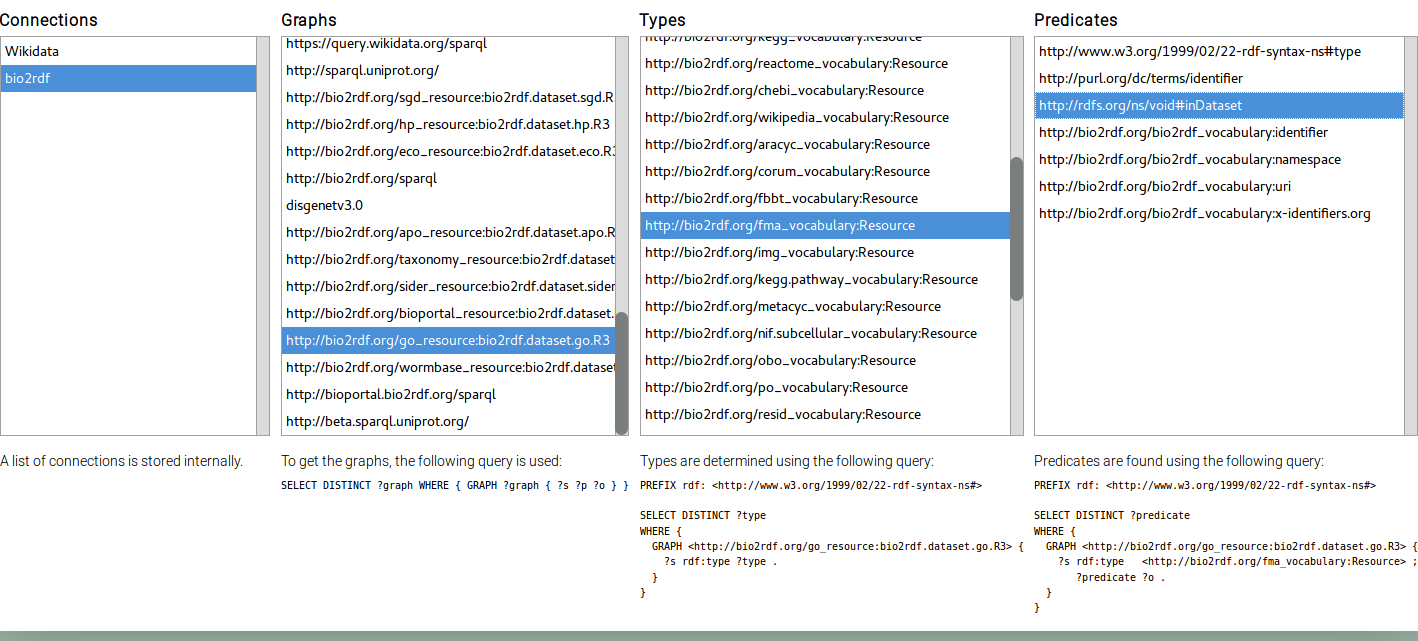
\includegraphics[width=1.0\textwidth]{figures/web-exploratory.png}
    \end{center}
    \caption{The \emph{exploratory} page enables users to learn about the
      structure of the triplets in a graph.}
    \label{fig:web-exploratory}
  \end{figure}

  The exploratory uses a common pattern in RDF to help writing queries.  Its
  interface provides a four-step selection process to find \emph{predicates}
  associated with an \texttt{rdf:type}.  The programs described in chapter
  \ref{chap:command-line} {\color{LinkGray}`\nameref{chap:command-line}'}
  automatically add the \texttt{rdf:type} annotations.

\subsection{Connections and graphs}

  The first step in finding predicates involves choosing a connection
  (see section \ref{sec:configure-connections} {\color{LinkGray}%
    `\nameref{sec:configure-connections}'}).  The second step involves
  choosing a graph.  If the connection does not support the use of graphs,
  the journey ends here.

\subsection{Types}

  The third step looks for triplets that match the pattern \emph{subject}
  $\rightarrow$ \texttt{rdf:type} $\rightarrow$ \emph{type}.  All matches for
  \emph{type} are displayed.  For data imported with \texttt{vcf2rdf} (see
  section \ref{sec:vcf2rdf} {\color{LinkGray}`\nameref{sec:vcf2rdf}'}), this
  will display (among other types) the \texttt{VariantCall} type.

\subsection{Predicates}

  Staying with the \texttt{VariantCall} example;  All data properties extracted
  from a VCF file can be found under this type.  A predicate displayed in this
  column occurs in \emph{at least} one triplet.  It not necessarily occurs in
  \emph{every} triplet.  Especially when using \texttt{INFO} and \texttt{FORMAT}
  fields in a VCF file, we recommend using them in a query inside an
  \texttt{OPTIONAL} clause.
